\documentclass[12pt,a4paper]{report}

% ------------------------------------------------
% PACKAGES
% ------------------------------------------------
\usepackage[utf8]{inputenc}
\usepackage[T1]{fontenc}
\usepackage[table]{xcolor}
\usepackage{geometry}
\usepackage{graphicx}
\usepackage{float}
\usepackage{array}
\usepackage{tabularx}
\usepackage{booktabs}
\usepackage{multirow}
\usepackage{tikz}
\usepackage[most]{tcolorbox}
\usepackage{setspace}
\usepackage{hyperref}
\usepackage{enumitem}
\usepackage{microtype}

\usetikzlibrary{arrows.meta, positioning, shapes.geometric, shapes.misc}

% ------------------------------------------------
% PAGE SETUP
% ------------------------------------------------
\geometry{margin=1in}
\onehalfspacing
\setlength{\parindent}{0pt}
\setlength{\parskip}{6pt}

% ------------------------------------------------
% COLOR THEME
% ------------------------------------------------
\definecolor{primary}{HTML}{4B2E83}
\definecolor{secondary}{HTML}{EDE7F6}
\definecolor{accent}{HTML}{00897B}
\definecolor{softteal}{HTML}{E0F2F1}
\definecolor{softcream}{HTML}{FFF8E1}
\definecolor{softgray}{HTML}{F5F5F5}
\definecolor{darkgray}{HTML}{333333}
\definecolor{nextstepblue}{HTML}{005BB5}

% ------------------------------------------------
% HYPERLINK SETUP
% ------------------------------------------------
\hypersetup{
    colorlinks=true,
    linkcolor=primary,
    urlcolor=nextstepblue,
    citecolor=accent
}

% ------------------------------------------------
% BOX STYLES
% ------------------------------------------------
\newtcolorbox{highlightBox}{
    colback=secondary,
    colframe=primary,
    boxrule=0.8pt,
    arc=2mm,
    left=8pt,
    right=8pt,
    top=6pt,
    bottom=6pt
}

\newtcolorbox{noteBox}{
    colback=softcream,
    colframe=accent,
    boxrule=0.8pt,
    arc=2mm,
    left=8pt,
    right=8pt,
    top=6pt,
    bottom=6pt
}

\begin{document}

\tableofcontents
\newpage

% ================================================================
% CHAPTER 3
% ================================================================
\chapter{Project Planning}

\section{Planning Introduction}

Project planning is a structured management process that defines the objectives, scope, schedule, resources, communication structure, and implementation strategy required for successful project execution. It provides a roadmap that guides the project team from initiation to deployment while ensuring that organisational goals, stakeholder expectations, and operational limitations remain aligned throughout the project lifecycle.

For technology integration projects, planning is especially important because such projects involve multiple connected activities, technical dependencies, resource limitations, and coordination among different stakeholder groups. Without proper planning, the implementation process may become delayed, responsibilities may become unclear, and the final system may fail to meet business expectations.

In the context of the Integrated Agency Management System (IAMS) project at NextStepBD, planning was necessary because the project aimed to replace fragmented operational practices with a centralized and integrated workflow environment. The proposed solution involved platform integration, process redesign, communication control, role-based access, and coordination between management, project managers, developers, operations staff, and clients.

The planning process for IAMS evolved through three major stages: the initial proposed plan, stakeholder discussion and evaluation, and the revised implementation plan. This iterative planning approach helped the project team move from a broad custom-development idea to a more practical SaaS-based integration strategy.

\begin{highlightBox}
\textbf{Planning Focus:} This chapter explains how the project plan was developed, reviewed, revised, and structured for implementation. It also presents the Work Breakdown Structure and Gantt Chart for the proposed IAMS implementation plan.
\end{highlightBox}

\section{Initial Proposed Plan}

The initial project proposal focused on developing a custom-built internal management system for NextStepBD. The main idea was to create a single proprietary platform that could centralize client communication, project management, task tracking, reporting, and developer coordination.

At this stage, the project was treated as a traditional software development initiative. The proposed plan included a dedicated database, a custom user interface, automated task assignment features, internal dashboards, and customized workflow automation. The system was expected to be designed and built mostly by NextStepBD's own development team.

Although the initial plan appeared technically possible, it introduced several important concerns. A fully custom system would require significant development time, testing effort, maintenance responsibility, and internal resource allocation. It could also reduce the availability of developers for billable client projects. Therefore, the initial plan required stakeholder review before implementation.

\begin{table}[H]
\centering
\renewcommand{\arraystretch}{1.35}
\begin{tabularx}{\textwidth}{|p{4cm}|X|}
\hline
\rowcolor{secondary}
\textbf{Initial Planning Area} & \textbf{Description} \\
\hline
Development Approach & Custom-built internal platform developed by the company’s own development team. \\
\hline
Core Components & Custom database, user interface, task assignment module, reporting dashboard, and workflow automation. \\
\hline
Expected Benefit & A centralized system fully customized for NextStepBD's internal workflow. \\
\hline
Major Concern & High development effort, longer implementation time, increased maintenance responsibility, and possible loss of billable developer hours. \\
\hline
\end{tabularx}
\caption{Summary of the Initial Proposed Plan}
\end{table}

\section{Stakeholder Discussion}

To evaluate the practicality of the initial proposal, a stakeholder strategy review was conducted involving the CEO, Project Manager, Coding Team Lead, development team representatives, and operations team members. The discussion focused on whether the custom-built system would be realistic, cost-effective, and suitable for the company’s current operational capacity.

During the discussion, the CEO expressed concern that building a fully custom enterprise platform would consume a large portion of the company’s billable developer hours. This would increase internal cost and delay return on investment. From a business perspective, the initial proposal was considered expensive compared to mature SaaS platforms already available in the market.

The Project Manager raised concerns about workflow governance and communication control. If clients were allowed unrestricted access to developer-level tasks and workflows, it could create scope creep, unstructured feedback, and operational disruption. Additionally, the Project Manager highlighted a significant risk to client satisfaction: removing informal, direct tools like WhatsApp might make clients feel disconnected or ignored. Therefore, the system needed a controlled communication structure that protected the internal team while ensuring clients still felt valued and heard.

The Coding Team Lead identified technical and architectural risks. The original proposal included automated task assignment based mainly on workload metrics, but this approach could not reliably consider developer specialization, task complexity, or contextual project knowledge. The need for a fully custom database was also questioned because platforms such as Jira already provide configurable workflow and issue management features.

\begin{noteBox}
\textbf{Stakeholder Outcome:} The stakeholder discussion changed the project direction from a custom software development plan to a SaaS-based integration plan. This change made the project more practical, faster to implement, and easier to maintain.
\end{noteBox}

\section{Revised Plan}

After stakeholder evaluation, the project strategy was revised from a fully custom development initiative into a SaaS-based integration project following a \textbf{Buy over Build} philosophy. Instead of building a monolithic internal platform, the revised plan proposed integrating existing enterprise tools that already support project tracking, issue management, communication, documentation, and development collaboration.

Under the revised approach, Jira Software would act as the \textbf{Single Source of Truth (SSOT)} for project and operational data. Jira Service Management would manage structured client communication and triage workflows. To directly address the concern regarding client satisfaction, JSM handles client interactions seamlessly via email integration, converting standard emails into managed tickets without forcing clients into a rigid portal if they prefer not to use it. Furthermore, clients gain explicit transparency through real-time status tracking on the portal, while informal text messaging is replaced by structured, high-touch weekly video syncs to maintain the personal relationship. Slack and GitHub would support internal collaboration and development automation. Confluence would be used for documentation and knowledge management, while automation tools would support workflow customization.

The revised plan reduced implementation complexity, development effort, project duration, and financial risk. It also preserved developer productivity by minimizing non-billable internal software development work. As a result, the final project planning framework became more realistic, scalable, and aligned with stakeholder expectations.

\begin{itemize}[leftmargin=*]
    \item Jira Software for centralized task and project tracking.
    \item Jira Service Management for structured client communication.
    \item Slack for team communication and notification flow.
    \item GitHub for development collaboration and version control.
    \item Confluence for documentation and knowledge base management.
    \item Automation tools for workflow customization.
\end{itemize}

\begin{figure}[H]
\centering
\resizebox{\textwidth}{!}{
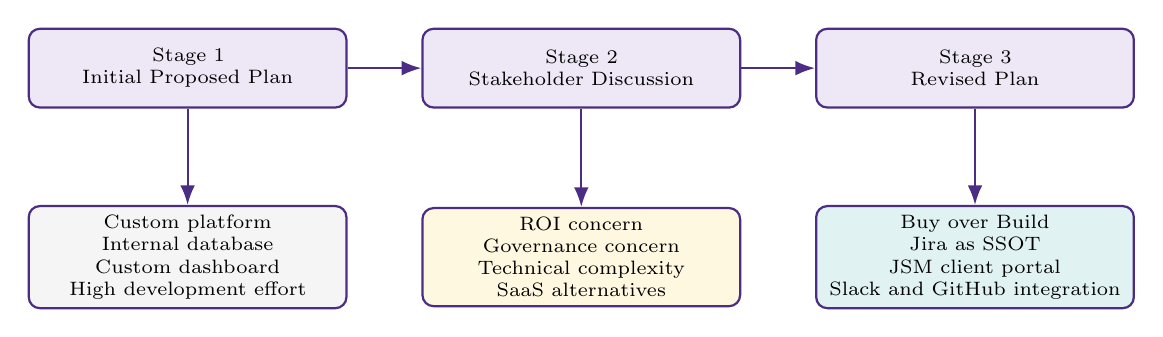
\begin{tikzpicture}[
    node distance=1.4cm,
    every node/.style={font=\scriptsize},
    stage/.style={
        rectangle,
        rounded corners,
        draw=primary,
        fill=secondary,
        thick,
        text width=3.8cm,
        minimum height=1cm,
        align=center
    },
    arrow/.style={thick, -{Latex[length=2.5mm]}, color=primary}
]

\node[stage] (s1) at (0,0) {Stage 1\\Initial Proposed Plan};
\node[stage] (s2) at (5,0) {Stage 2\\Stakeholder Discussion};
\node[stage] (s3) at (10,0) {Stage 3\\Revised Plan};

\draw[arrow] (s1) -- (s2);
\draw[arrow] (s2) -- (s3);

\node[stage, fill=softgray] (d1) at (0,-2.4)
{Custom platform\\Internal database\\Custom dashboard\\High development effort};

\node[stage, fill=softcream] (d2) at (5,-2.4)
{ROI concern\\Governance concern\\Technical complexity\\SaaS alternatives};

\node[stage, fill=softteal] (d3) at (10,-2.4)
{Buy over Build\\Jira as SSOT\\JSM client portal\\Slack and GitHub integration};

\draw[arrow] (s1) -- (d1);
\draw[arrow] (s2) -- (d2);
\draw[arrow] (s3) -- (d3);

\end{tikzpicture}
}
\caption{Evolution of the IAMS project planning strategy}
\end{figure}

\begin{table}[H]
\centering
\renewcommand{\arraystretch}{1.35}
\small
\begin{tabularx}{\textwidth}{|p{4cm}|X|X|}
\hline
\rowcolor{secondary}
\textbf{Planning Area} & \textbf{Initial Proposed Plan} & \textbf{Revised Integration Plan} \\
\hline
Development Approach & Custom-built internal platform & SaaS integration architecture \\
\hline
Core Technology & Custom database and application & Jira, JSM, Slack, GitHub, Confluence \\
\hline
Project Duration & Estimated 6--12 months & Shorter phased deployment \\
\hline
Development Effort & Full-scale software development & Configuration and integration \\
\hline
Developer Resource Usage & Heavy internal resource consumption & Minimal disruption to billable work \\
\hline
Workflow Management & Custom workflow implementation & Jira-based workflow automation \\
\hline
Client Communication & Direct system interaction & Structured JSM portal \\
\hline
Maintenance Responsibility & Fully internal maintenance & Vendor-supported SaaS ecosystem \\
\hline
ROI Outlook & Delayed and uncertain & Faster and more predictable \\
\hline
\end{tabularx}
\caption{Comparison between the initial proposed plan and the revised integration plan}
\end{table}

\begin{figure}[H]
\centering
\resizebox{0.9\textwidth}{!}{
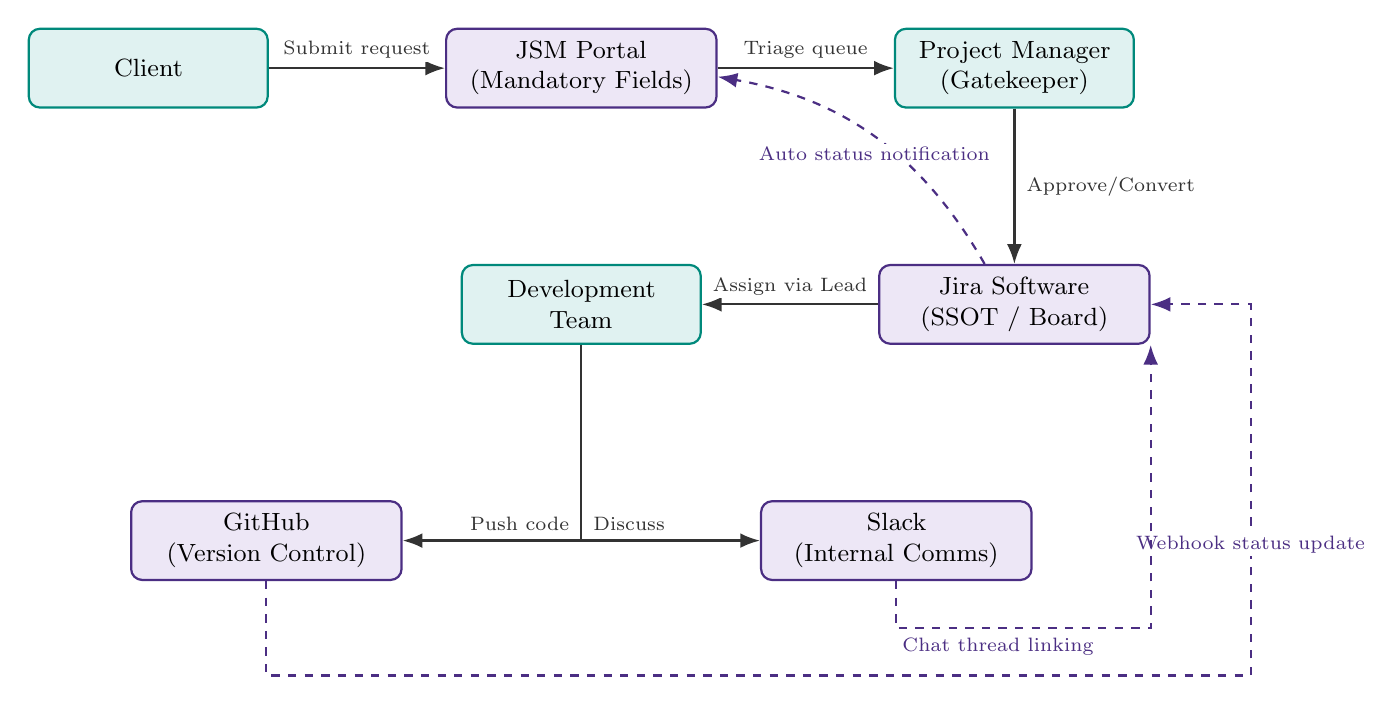
\begin{tikzpicture}[
    node distance=2cm,
    every node/.style={font=\small},
    actor/.style={rectangle, rounded corners, draw=accent, fill=softteal, thick, text width=2.8cm, align=center, minimum height=1cm},
    system/.style={rectangle, rounded corners, draw=primary, fill=secondary, thick, text width=3.2cm, align=center, minimum height=1cm},
    arrow/.style={thick, -{Latex[length=2.5mm]}, color=darkgray}
]

% Nodes
\node[actor] (client) at (0,0) {Client};
\node[system] (jsm) at (5.5,0) {JSM Portal\\(Mandatory Fields)};
\node[actor] (pm) at (11,0) {Project Manager\\(Gatekeeper)};

\node[system] (jira) at (11,-3) {Jira Software\\(SSOT / Board)};
\node[actor] (dev) at (5.5,-3) {Development\\Team};

\node[system] (git) at (1.5,-6) {GitHub\\(Version Control)};
\node[system] (slack) at (9.5,-6) {Slack\\(Internal Comms)};

% Arrows (Direct flows)
\draw[arrow] (client) -- node[midway, above=2pt, fill=white, inner sep=1pt] {\scriptsize Submit request} (jsm);
\draw[arrow] (jsm) -- node[midway, above=2pt, fill=white, inner sep=1pt] {\scriptsize Triage queue} (pm);
\draw[arrow] (pm) -- node[midway, right=3pt, fill=white, inner sep=1pt] {\scriptsize Approve/Convert} (jira);
\draw[arrow] (jira) -- node[midway, above=2pt, fill=white, inner sep=1pt] {\scriptsize Assign via Lead} (dev);

\draw[arrow] (dev) |- node[midway, left=3pt, yshift=6pt, fill=white, inner sep=1pt] {\scriptsize Push code} (git);
\draw[arrow] (dev) |- node[midway, right=3pt, yshift=6pt, fill=white, inner sep=1pt] {\scriptsize Discuss} (slack);

% Arrows (Automated Webhooks - dashed)
\draw[arrow, dashed, color=primary] (git.south) -- ++(0,-1.2) -- ++(12.5,0) |- node[pos=0.2, left=12pt, below=2pt, fill=white, inner sep=1pt] {\scriptsize Webhook status update} (jira.east);
\draw[arrow, dashed, color=primary] (slack.south) -- ++(0,-0.6) -| node[pos=0.2, below=2pt, fill=white, inner sep=1pt] {\scriptsize Chat thread linking} (jira.south east);

% Return notification to JSM
\draw[arrow, dashed, color=primary] (jira) to[bend right=25] node[midway, left=12pt, below=2pt,  fill=white, inner sep=1pt] {\scriptsize Auto status notification} (jsm);

\end{tikzpicture}
}
\caption{Conceptual workflow of the SaaS integration showing tool linkages and user boundaries}
\end{figure}

\section{Problem Resolution Mapping}

The revised SaaS integration plan was specifically designed to resolve the five core operational problems identified during the initial system analysis phase. By moving to a connected ecosystem, the architecture actively dismantles previous bottlenecks. Table 3.3 illustrates exactly how the new system addresses and resolves each of the legacy system failures.

\begin{table}[H]
\centering
\renewcommand{\arraystretch}{1.4}
\small
\begin{tabularx}{\textwidth}{|p{4.5cm}|X|}
\hline
\rowcolor{secondary}
\textbf{Identified Problem} & \textbf{Resolution in the Revised Plan} \\
\hline
\textbf{1. Fragmented System Architecture} \newline Data scattered across WhatsApp, Excel, and GitHub. & \textbf{Jira as Single Source of Truth (SSOT):} Native APIs and integrated webhooks connect Slack and GitHub directly into Jira, centralizing all project data and eliminating manual data transfer. \\
\hline
\textbf{2. PM Bottleneck} \newline The PM acts as the sole manual bridge between clients and developers. & \textbf{JSM Triage Dashboard:} Automation routes client requests into a defined queue. The PM simply acts as a fast gatekeeper, instantly converting valid requests into developer tickets alongside smart capacity recommendations for developer assignment. \\
\hline
\textbf{3. Unstructured Requirements} \newline Scope creep caused by informal texting and missing details. & \textbf{Mandatory Portal Fields:} The JSM portal requires structured inputs (e.g., reproduction steps, environment details). Furthermore, "dual-channel" communication isolates developers in Slack, shielding them from client noise and sudden scope changes. \\
\hline
\textbf{4. Lack of Centralized Tracking} \newline No visibility into exact task status or project health. & \textbf{Live Jira Boards:} Configured Kanban boards and dashboards provide real-time tracking for the internal team, while clients gain transparency through the portal status tracker without needing to ask for updates. \\
\hline
\textbf{5. Security \& Quality Risks} \newline Sharing credentials via chat and untracked code deployments. & \textbf{Role-Based Access Control (RBAC):} Strict permission tiers ensure clients and unauthorized staff cannot access sensitive IP or billing data. Automated GitHub webhooks link code commits directly to tickets for complete auditability. \\
\hline
\end{tabularx}
\caption{Mapping of identified core problems to specific SaaS integration solutions}
\end{table}

\section{Work Breakdown Structure}

The Work Breakdown Structure (WBS) divides the IAMS project into smaller and manageable work packages. It helps the project team understand deliverables, assign responsibilities, monitor progress, and control implementation activities step by step.

For the NextStepBD IAMS project, the WBS is organized into six major phases: discovery and requirements, system architecture and design, development and integration, testing and review, training and pilot launch, and full deployment with optimization. This structure ensures that each part of the project can be tracked independently while still contributing to the overall implementation objective.

\begin{figure}[H]
\centering
\resizebox{\textwidth}{!}{
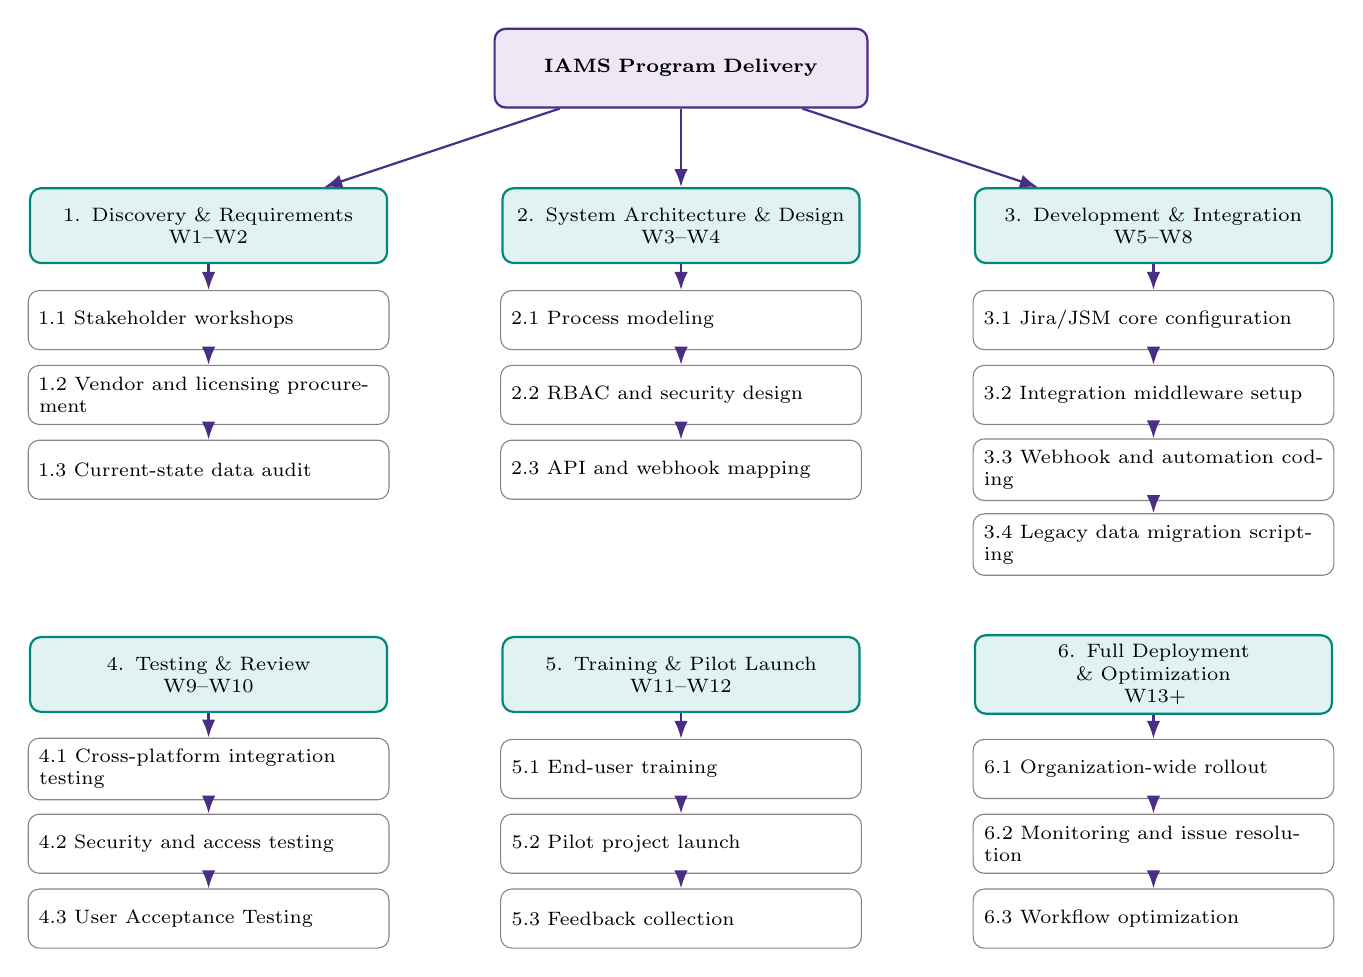
\begin{tikzpicture}[
    every node/.style={font=\scriptsize},
    root/.style={
        rectangle,
        rounded corners,
        draw=primary,
        fill=secondary,
        thick,
        text width=4.5cm,
        minimum height=1cm,
        align=center
    },
    phase/.style={
        rectangle,
        rounded corners,
        draw=accent,
        fill=softteal,
        thick,
        text width=4.3cm,
        minimum height=0.95cm,
        align=center
    },
    task/.style={
        rectangle,
        rounded corners,
        draw=darkgray!60,
        fill=white,
        text width=4.3cm,
        minimum height=0.75cm,
        align=left,
        inner sep=4pt
    },
    arrow/.style={thick, -{Latex[length=2.3mm]}, color=primary}
]

% Root
\node[root] (root) at (0,0) {\textbf{IAMS Program Delivery}};

% Top-row phases
\node[phase] (p1) at (-6,-2) {1. Discovery \& Requirements\\W1--W2};
\node[phase] (p2) at (0,-2) {2. System Architecture \& Design\\W3--W4};
\node[phase] (p3) at (6,-2) {3. Development \& Integration\\W5--W8};

% Bottom-row phases
\node[phase] (p4) at (-6,-7.7) {4. Testing \& Review\\W9--W10};
\node[phase] (p5) at (0,-7.7) {5. Training \& Pilot Launch\\W11--W12};
\node[phase] (p6) at (6,-7.7) {6. Full Deployment \& Optimization\\W13+};

% Root arrows (Top Row)
\draw[arrow] (root) -- (p1);
\draw[arrow] (root) -- (p2);
\draw[arrow] (root) -- (p3);

% Phase 1 tasks
\node[task] (p1a) at (-6,-3.2) {1.1 Stakeholder workshops};
\node[task] (p1b) at (-6,-4.15) {1.2 Vendor and licensing procurement};
\node[task] (p1c) at (-6,-5.1) {1.3 Current-state data audit};

% Phase 2 tasks
\node[task] (p2a) at (0,-3.2) {2.1 Process modeling};
\node[task] (p2b) at (0,-4.15) {2.2 RBAC and security design};
\node[task] (p2c) at (0,-5.1) {2.3 API and webhook mapping};

% Phase 3 tasks
\node[task] (p3a) at (6,-3.2) {3.1 Jira/JSM core configuration};
\node[task] (p3b) at (6,-4.15) {3.2 Integration middleware setup};
\node[task] (p3c) at (6,-5.1) {3.3 Webhook and automation coding};
\node[task] (p3d) at (6,-6.05) {3.4 Legacy data migration scripting};

% Phase 4 tasks
\node[task] (p4a) at (-6,-8.9) {4.1 Cross-platform integration testing};
\node[task] (p4b) at (-6,-9.85) {4.2 Security and access testing};
\node[task] (p4c) at (-6,-10.8) {4.3 User Acceptance Testing};

% Phase 5 tasks
\node[task] (p5a) at (0,-8.9) {5.1 End-user training};
\node[task] (p5b) at (0,-9.85) {5.2 Pilot project launch};
\node[task] (p5c) at (0,-10.8) {5.3 Feedback collection};

% Phase 6 tasks
\node[task] (p6a) at (6,-8.9) {6.1 Organization-wide rollout};
\node[task] (p6b) at (6,-9.85) {6.2 Monitoring and issue resolution};
\node[task] (p6c) at (6,-10.8) {6.3 Workflow optimization};

% Arrows for tasks
\draw[arrow] (p1) -- (p1a);
\draw[arrow] (p1a) -- (p1b);
\draw[arrow] (p1b) -- (p1c);

\draw[arrow] (p2) -- (p2a);
\draw[arrow] (p2a) -- (p2b);
\draw[arrow] (p2b) -- (p2c);

\draw[arrow] (p3) -- (p3a);
\draw[arrow] (p3a) -- (p3b);
\draw[arrow] (p3b) -- (p3c);
\draw[arrow] (p3c) -- (p3d);

\draw[arrow] (p4) -- (p4a);
\draw[arrow] (p4a) -- (p4b);
\draw[arrow] (p4b) -- (p4c);

\draw[arrow] (p5) -- (p5a);
\draw[arrow] (p5a) -- (p5b);
\draw[arrow] (p5b) -- (p5c);

\draw[arrow] (p6) -- (p6a);
\draw[arrow] (p6a) -- (p6b);
\draw[arrow] (p6b) -- (p6c);

\end{tikzpicture}
}
\caption{Work Breakdown Structure for the IAMS implementation plan}
\end{figure}

\section{Gantt Chart}

A Gantt Chart is used to present the project schedule visually by showing activities, durations, and implementation phases over time. For the IAMS project, the schedule follows a phased approach so that NextStepBD can gradually adopt the new system without disrupting ongoing client work.

The implementation plan begins with discovery and requirements, followed by system design, development and integration, testing, training, pilot launch, and final deployment. It is important to note that while the initial prototyping and pilot sandbox are designed to be operational within the first four to five weeks, the extended 13-week schedule accounts for full organizational migration, comprehensive training, and final optimization safely alongside active client workloads. This schedule allows the project team to review progress continuously and make corrections before full-scale adoption.

\begin{table}[H]
\centering
\renewcommand{\arraystretch}{1.25}
\small
\begin{tabularx}{\textwidth}{|p{4.6cm}|c|c|c|c|}
\hline
\rowcolor{secondary}
\textbf{Project Activity} & \textbf{Weeks 1--4} & \textbf{Weeks 5--8} & \textbf{Weeks 9--12} & \textbf{Week 13+} \\
\hline
Discovery and Requirements & \cellcolor{accent!55} & & & \\
\hline
Stakeholder Workshops & \cellcolor{accent!35} & & & \\
\hline
Vendor and Licensing Procurement & \cellcolor{accent!35} & & & \\
\hline
System Architecture and Design & \cellcolor{primary!25} & \cellcolor{primary!45} & & \\
\hline
RBAC and Security Design & & \cellcolor{primary!35} & & \\
\hline
API and Webhook Mapping & & \cellcolor{primary!35} & & \\
\hline
Development and Integration & & \cellcolor{nextstepblue!35} & \cellcolor{nextstepblue!55} & \\
\hline
Jira/JSM Core Configuration & & \cellcolor{nextstepblue!30} & & \\
\hline
Webhook and Automation Coding & & & \cellcolor{nextstepblue!45} & \\
\hline
Testing and Review & & & \cellcolor{accent!25} & \\
\hline
Training and Pilot Launch & & & \cellcolor{accent!20} & \cellcolor{accent!40} \\
\hline
Full Deployment and Optimization & & & & \cellcolor{primary!45} \\
\hline
\end{tabularx}
\caption{Gantt Chart for the IAMS implementation schedule}
\end{table}

\section{Resource and Cost Allocation}

The transition from a custom-built platform to a SaaS integration model drastically shifts the financial and resource planning strategy. Rather than allocating capital toward thousands of internal billable hours for developing, testing, and maintaining proprietary software, NextStepBD will invest in monthly licensing fees for enterprise tools. 

The primary cost variables involve purchasing additional \textbf{Jira Software} developer seats, \textbf{Jira Service Management (JSM)} agent licenses for the Project Managers, and a potential upgrade to \textbf{Slack} business tiers for advanced webhook retention. However, this recurring operational expense is vastly outweighed by the preservation of billable developer capacity. The internal resource allocation is restricted to a brief configuration period (principally by operations and architecture leads) rather than engaging the core coding team in non-revenue-generating internal development.

\section{Risk Management}

While integrating mature SaaS platforms mitigates the technical risks of custom development, it introduces new operational and adoption risks that must be managed:

\begin{itemize}[leftmargin=*]
    \item \textbf{User Resistance to Process Change:} Both clients and developers are accustomed to the informal speed of WhatsApp. To mitigate this risk, NextStepBD will implement communication mandates explicitly disabling WhatsApp for work requests, paired with hands-on training sessions highlighting the time-saving benefits of Jira.
    \item \textbf{Integration Failure:} Relying heavily on webhooks between Jira, Slack, and GitHub presents a single point of failure if APIs change or tokens expire. Mitigation involves establishing monitoring toolsets within Jira to alert administrators immediately when webhook synchronizations fail.
    \item \textbf{Licensing Scope Creep:} If access controls are loosely managed, the company may accidentally provision expensive JSM agent licenses to standard developers. This is mitigated through strict, script-enforced Role-Based Access Control (RBAC).
\end{itemize}

\section{Conclusion}

This chapter described the planning process for the proposed IAMS project at NextStepBD. The planning process began with an initial custom software development proposal, but stakeholder discussion revealed concerns related to development time, technical complexity, workflow governance, and long-term maintenance. As a result, the project plan was revised into a SaaS-based integration strategy using Jira, Jira Service Management, Slack, GitHub, Confluence, and automation tools.

The revised plan is more practical for NextStepBD because it reduces development workload, shortens implementation time, minimizes implementation risk, and supports a controlled workflow structure. The Work Breakdown Structure divides the project into manageable work packages, while the Gantt Chart provides a phased timeline for implementation. Overall, this chapter shows that successful system development depends not only on technical feasibility but also on careful planning, stakeholder involvement, and realistic implementation strategy.

\end{document}
